\section{Introduction des Solutions}
\label{introSolutions}
	Le travail effectué dans Blue Banana (cf \ref{BlueBanana}, page \pageref{BlueBanana}) s'intéresse à une partie du jeu bien définie, qui est les déplacements entre les zones denses. Durant le stage, il a donc fallu cherché des solutions qui permettraient d'améliorer le travail existant. Plusieurs pistes de solution ont été trouvé, deux de ces pistes ont été implémentées et testées. Les deux solutions implémentées, durant le stage, sont la mise en place d'un cache pour les zones denses de l'environnement, et la modification du rapatriement des données qui était réalisé dans Blue Banana, pour les déplacements entre les zones denses.
\par Dans la première solution, l'intérêt s'est porté sur une partie du jeu qui n'était pas étudiée dans Blue Banana. Le comportement des avatars dans les zones denses restait le même que dans Solipsis, nous avons donc décidé d'améliorer le fonctionnent dans ces zones denses.A l'intérieur de celles-ci, les joueurs se déplacent de façon désordonnée et bougent la plupart du temps dans un secteur restreint. L'utilisation d'un cache est alors apparu comme une solution d'amélioration évidente. Le principe du cache est très simple, un nœud oubliait des voisins dont il pourrait avoir besoin dans un futur plus ou moins proche (en fonction de la mobilité dans le jeu), la mise en place du cache va permettre de garder un nombre \textit{N} de nœuds dans l'éventualité où le nœud revienne dans une zone où il ai déjà venu (voir Schéma \ref{mouveDense}). Nous expliquerons les différentes solutions que nous avons testé pour le cache, et pourquoi celles que nous avons retenu fonctionnaient mieux.
	\vspace{5mm}
        \begin{figure}[!h]
        \centering
        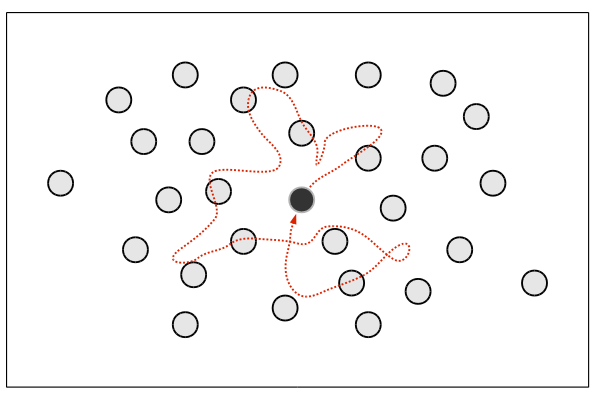
\includegraphics[scale=0.45]{./Ressources/Images/mouvementsZoneDense.png}\\
        \caption{Exemple d'une trajectoire d'un joueur dans une zone dense}
        \label{mouveDense}
        \end{figure}
\par La deuxième solution a consisté à modifier le rapatriement des données réalisé dans Blue Banana, pour que celui-ci se fasse de manière plus fine. Les modification que nous avons introduites doivent permettre d'économiser des messages et d'améliorer la cohérence de la topologie. Différentes techniques et algorithmes ont été testés, les plus importantes seront décrites et expliquées.
 
\begin{table}[!h]
  \begin{center}
    \begin{tabular}{|c|c|c|}
      \hline
      Solution & Partie Améliorée & Gains\\
      \hline
      Introduction d'un cache  & Dans les zones denses & - de msg, + cohérence de la topologie \\
      Amélioration du rapatriement & Entre les zones denses & - de msg, + cohérence de la topologie\\
      \hline
    \end{tabular}
  \end{center}
  \label{tab:config2}
  \caption{Tableau récapitulatif des solutions ajoutées durant le stage}
\end{table}


\subsection{Le modèle de mobilité}

Un modèle de mobilité a été mis en place dans Blue Banana, nous allons le présenter car il est utilisé pour les différents tests réalisés pour les solutions mises en place. Pour cela, un degré de mobilité à un instant donné, a été introduit. Il s'agit du nombre d'avatars dans l'état \textbf{T}(ravelling) à cet instant sur le nombre total d'avatars. Le modèle de mobilité implémenté dans Blue Banana se base sur l'automate (cf partie~\ref{Automate}). A intervalles réguliers, PeerSim décide si un avatar doit ou non changer d'état. Il réalise ceci grâce aux différentes probabilités présentées dans les fichiers de configurations. A chaque fois qu'un déplacement est décidé, une destination est choisie. L'avatar commence alors son déplacement, chaque mouvement est rectiligne mais non uniforme (car accélération). L'accélération est nulle lorsque la vitesse maximale est atteinte, cette vitesse maximale est choisie en fonction de la zone où se trouve l'avatar.


\par L'automate étant mis à jour toutes les 100ms, même un petit changement dans les probabilités, peut entrainer des gros changements sur la mobilité. La transition WtoT a été choisie, dans Blue Banana, pour faire varier la mobilité. Cette transition permet de déclencher le passage d'un avatar d'un état d'exploration désordonné à un état de déplacement rapide. Sur la figure~\ref{fig:mobility}, nous pouvons voir les différentes valeurs affectées à la transition et les degrés de mobilité correspondants. 

\begin{figure}
  \begin{center}
    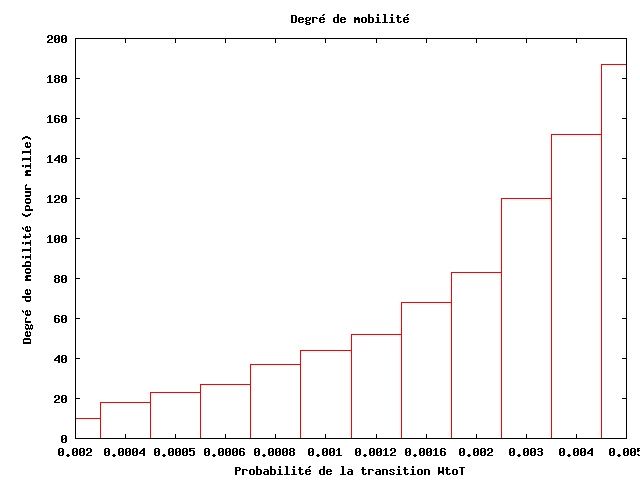
\includegraphics[scale=0.40]{./Ressources/Images/mobility.png} \\
    \caption{\textit{\small Influence du changement de probabilité sur
        la transition WtoT de l'automate sur le degré de mobilité du
        Métavers}}
    \label{fig:mobility}
  \end{center}
\end{figure}




